\documentclass{beamer}
\usepackage[utf8]{inputenc}
\usepackage[brazil]{babel}
\usepackage{hyperref}
\usepackage{graphicx}
\usepackage{utopia} %font utopia imported

\graphicspath{{./imagens/sumario/}}

\hypersetup{
    colorlinks=true,
    linkcolor=blue,
    filecolor=magenta,      
    urlcolor=cyan,
}

\usetheme{Berkeley}
\usecolortheme{default}

%------------------------------------------------------------
%This block of code defines the information to appear in the
%Title page
\title[LDO] %optional
{\textbf{Trabalho LDO}}

\subtitle{\textbf{Um breve ínicio em Aprendizado de Máquina}}

\institute[PUC] % (optional)
{
  \inst{1}%
  \emph{Pontifícia Universidade Católica de Minas Gerais}
  \\PUC-MG
}

\date[2020] % (optional)
{Novembro 2020}

%End of title page configuration block
%------------------------------------------------------------



%------------------------------------------------------------
%The next block of commands puts the table of contents at the 
%beginning of each section and highlights the current section:

%\AtBeginSection[]
%{
%  \begin{frame}
%    \frametitle{Cronograma}
%    \tableofcontents[currentsection]
%  \end{frame}
%}
%------------------------------------------------------------


\begin{document}

%The next statement creates the title page.
\frame{\titlepage}


%---------------------------------------------------------
%This block of code is for the table of contents after
%the title page
\begin{frame}
    \frametitle{Cronograma}
    \tableofcontents
\end{frame}
%---------------------------------------------------------

\section{O que é Machine Learning?}

%---------------------------------------------------------
\begin{frame}

    \begin{figure}[ht]
        \centering
        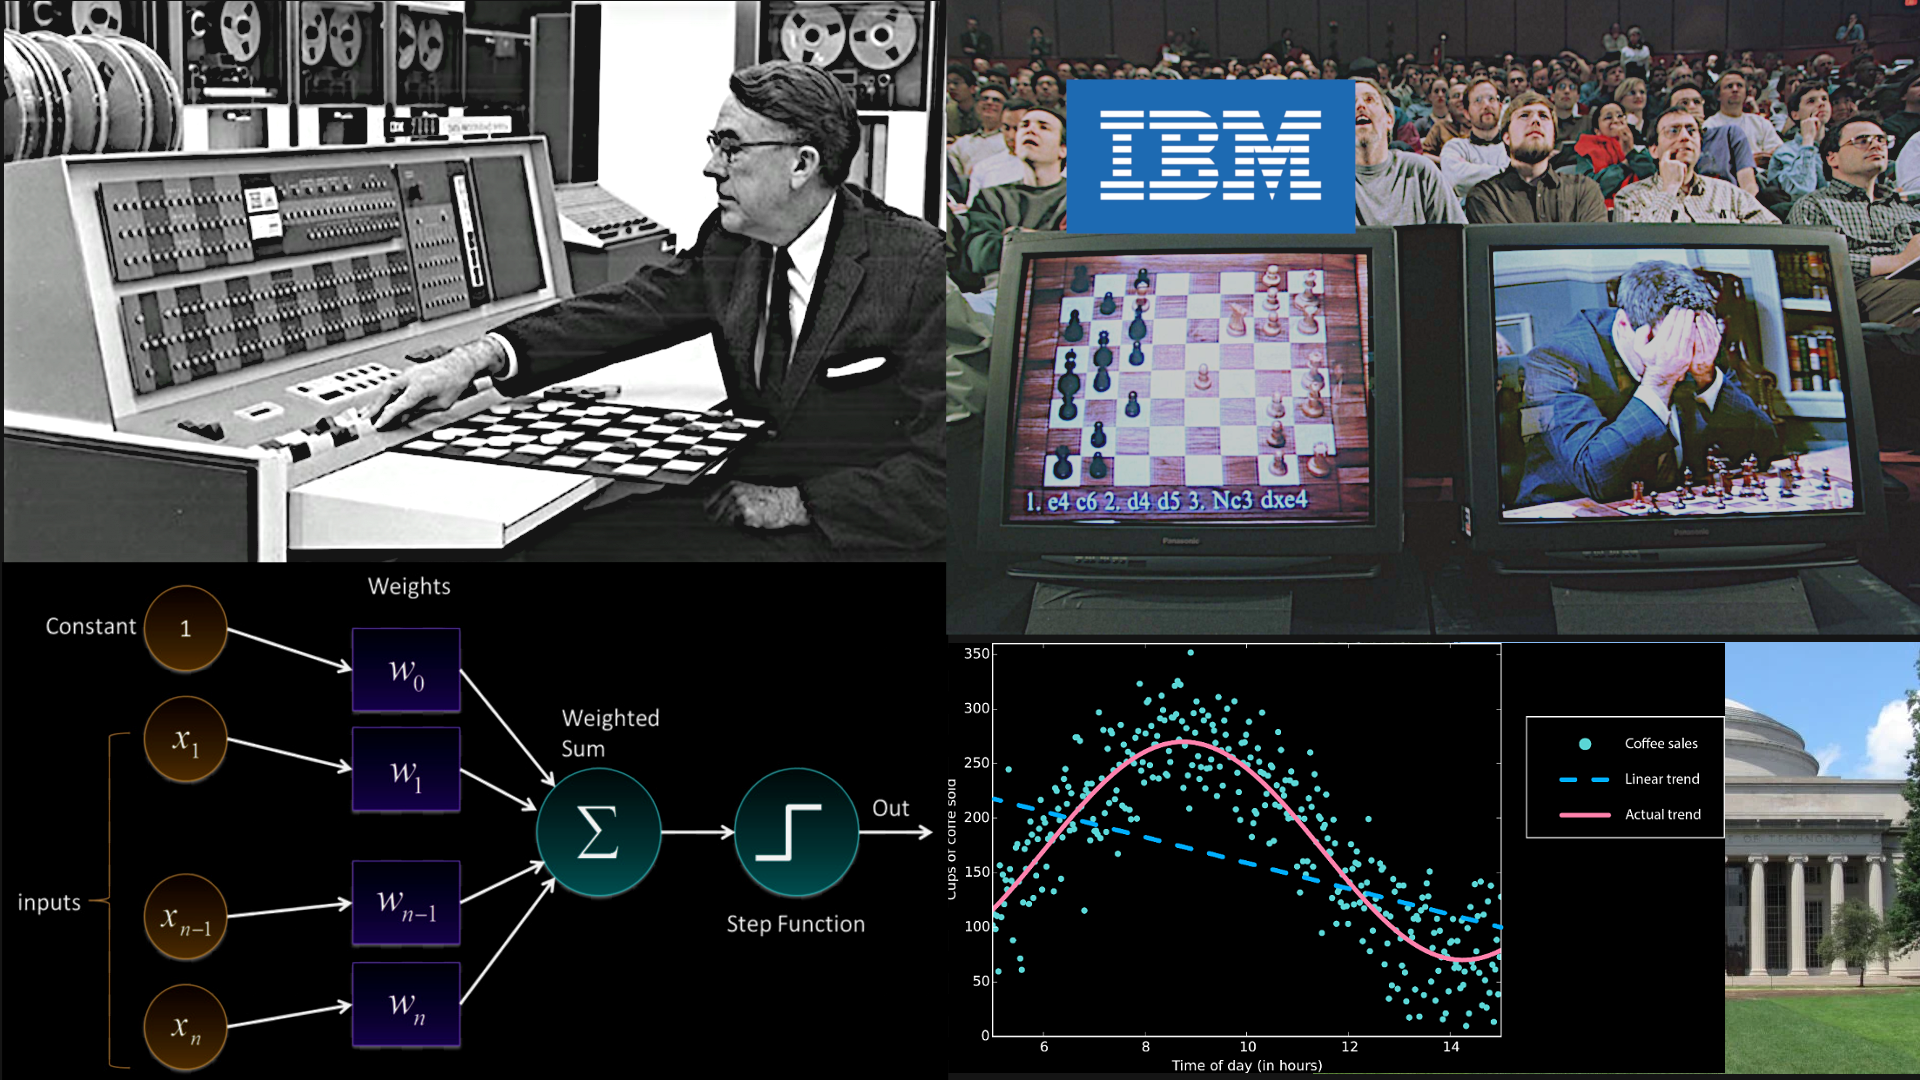
\includegraphics[scale=0.5]{Capitulo1.png}
        \caption{\href{run:./capitulos/Capitulo_01/Capitulo1.pdf}{Link para o capítulo I}}
    \end{figure}

\end{frame}
%---------------------------------------------------------
%FIM DE SEÇÃO
%---------------------------------------------------------

\section{Novidades}

%---------------------------------------------------------
\begin{frame}

    \begin{figure}[ht]
        \centering
        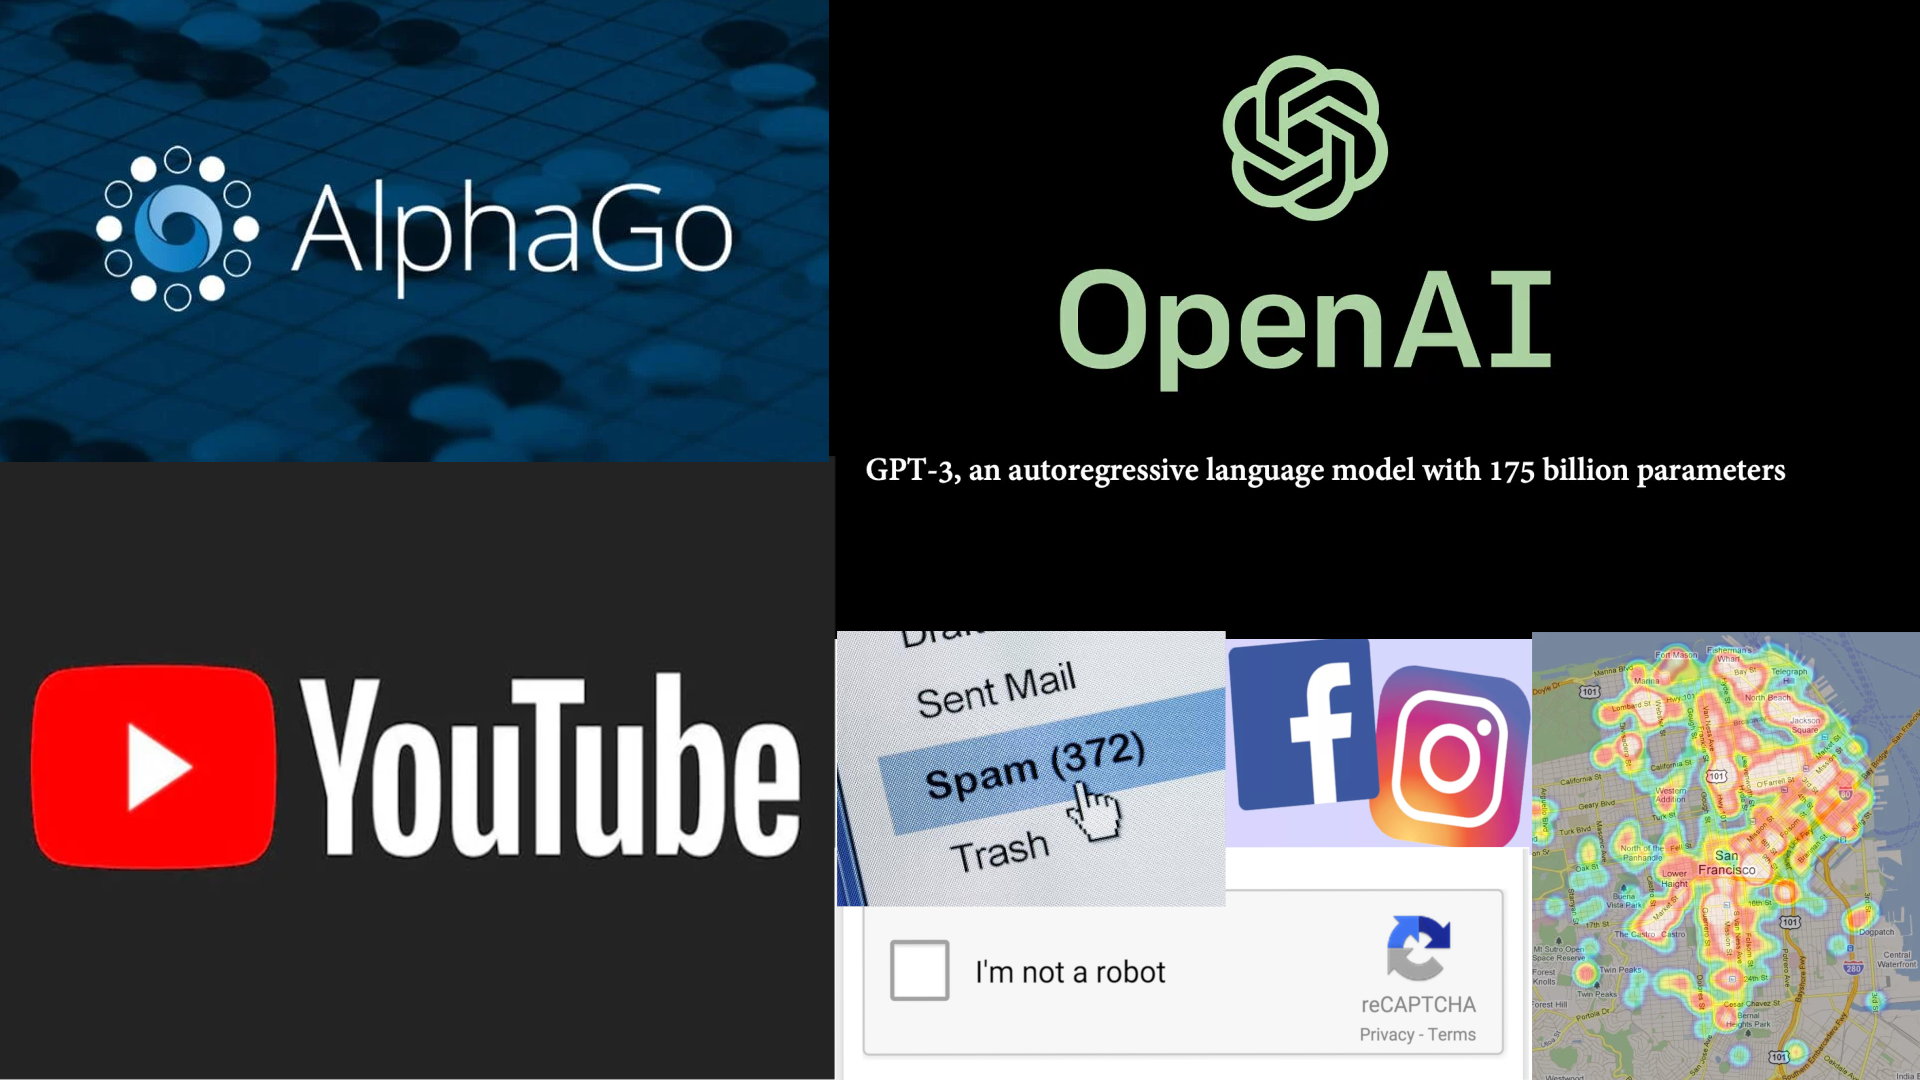
\includegraphics[scale=0.5]{Capitulo2.png}
        \caption{\href{run:./capitulos/Capitulo_02/Capitulo2.pdf}{Link para o capítulo II}}
    \end{figure}

\end{frame}
%---------------------------------------------------------

\section{Como o aprendizado acontece?}

%---------------------------------------------------------
%Two columns
\begin{frame}

    \begin{figure}[ht]
        \centering
        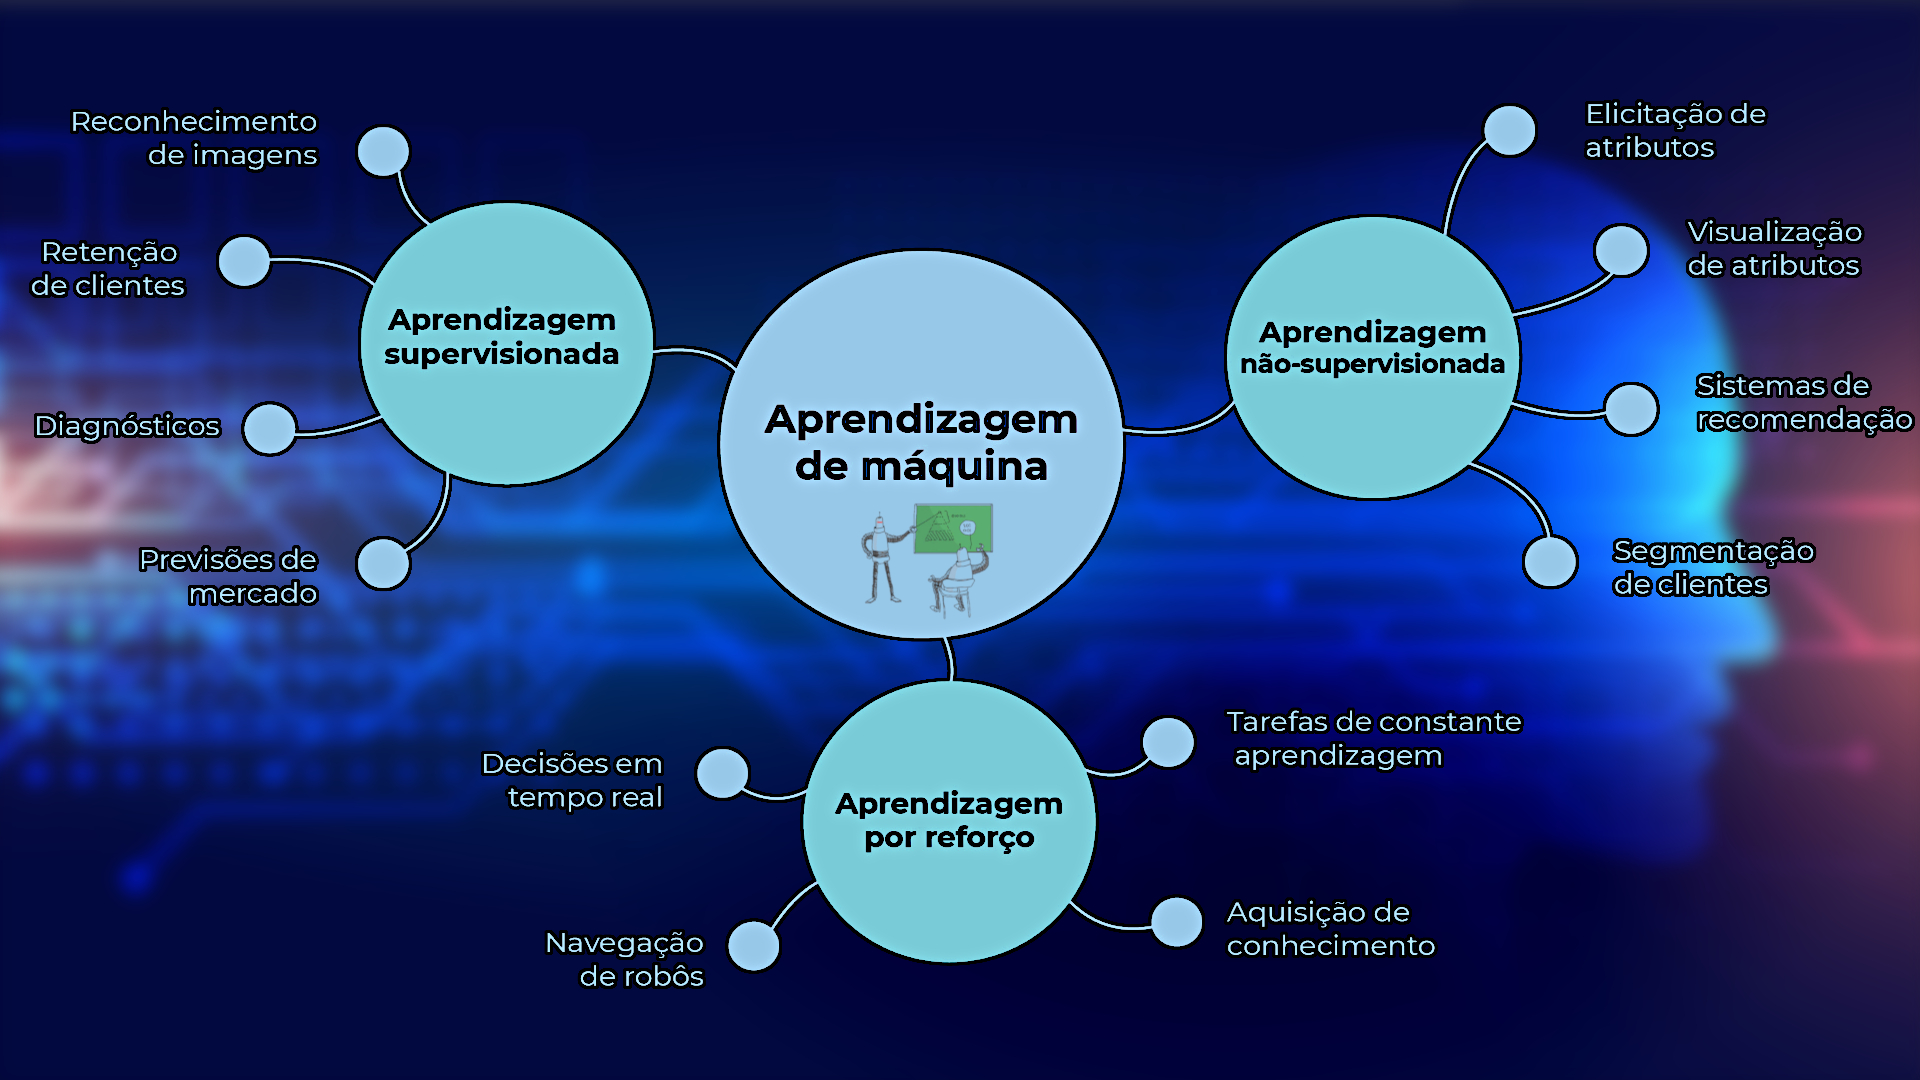
\includegraphics[scale=0.5]{Capitulo3.png}
        \caption{\href{run:./capitulos/Capitulo_03/Capitulo03.pdf}{Link para o capítulo III}}
    \end{figure}

\end{frame}
%---------------------------------------------------------

\section{Tópicos de Machine Learning}

%---------------------------------------------------------
\begin{frame}

    \begin{figure}[ht]
        \centering
        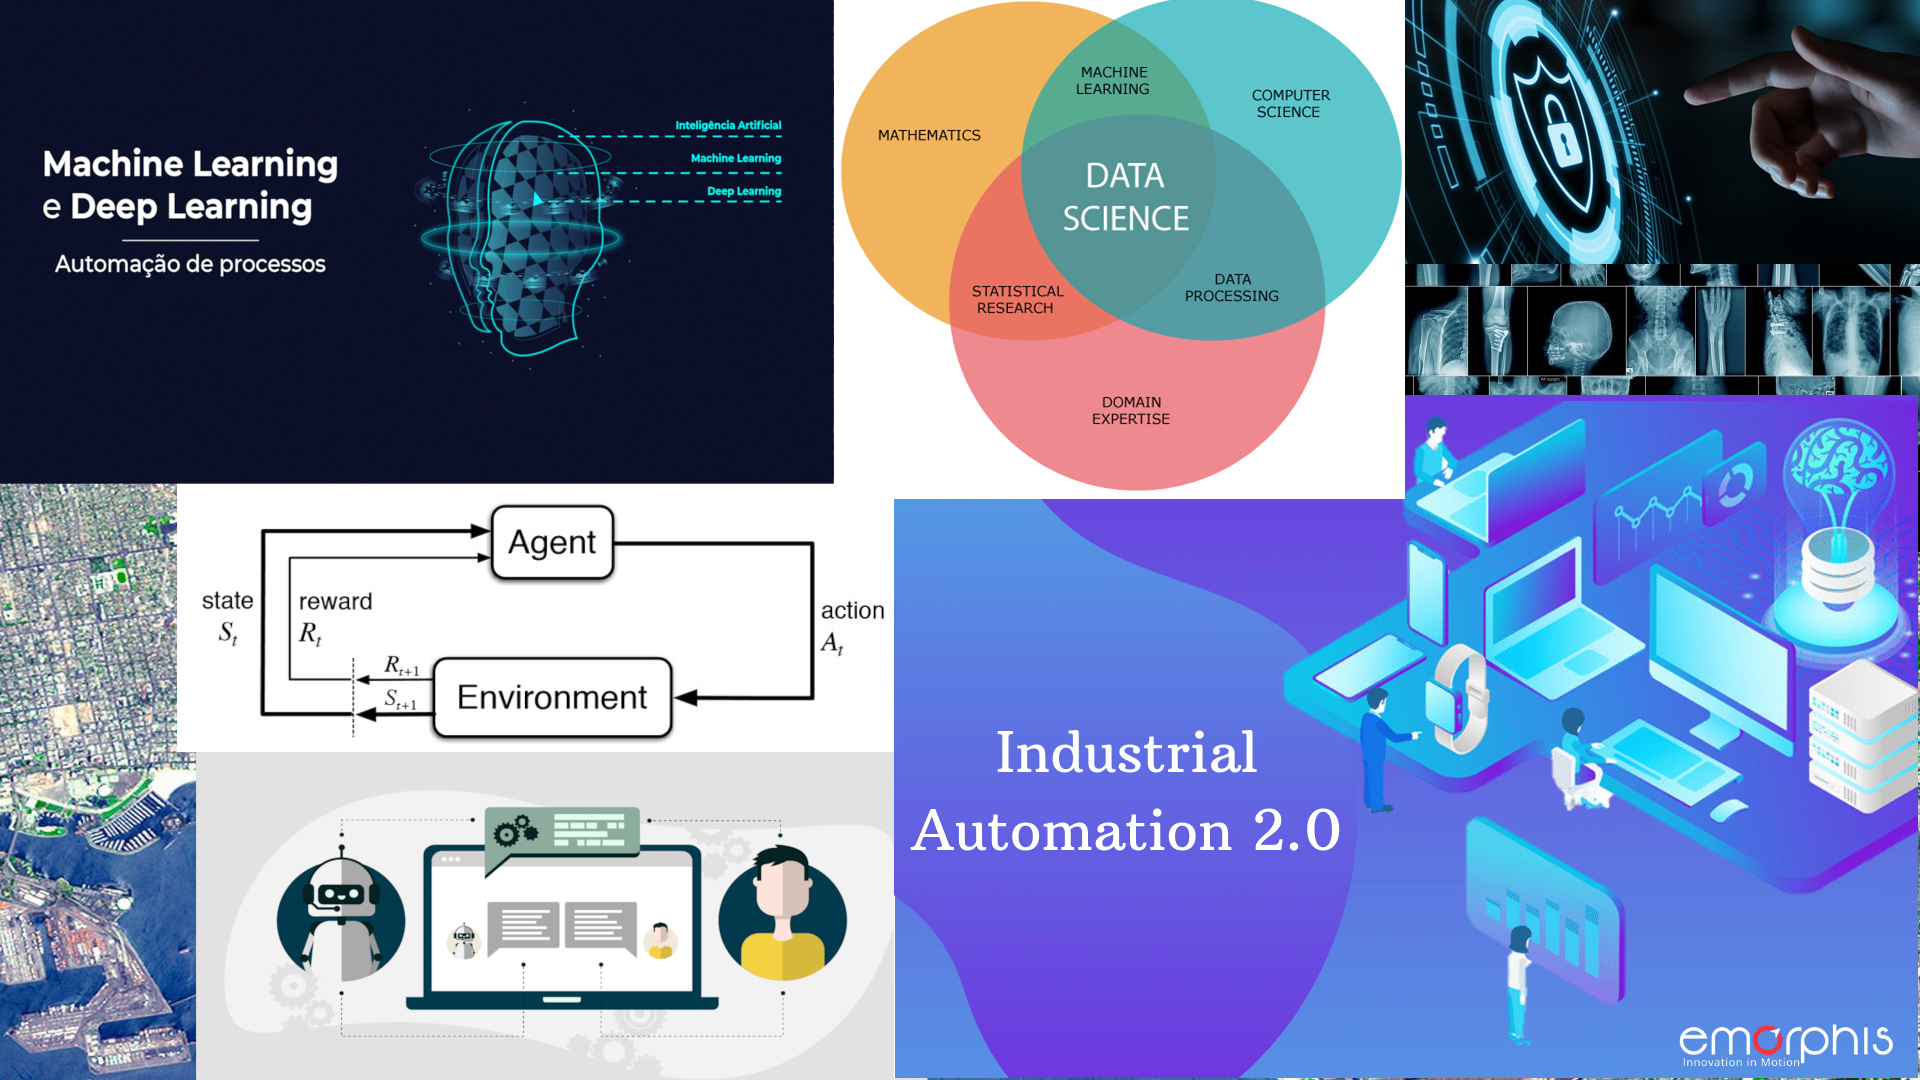
\includegraphics[scale=0.5]{Capitulo4.png}
        \caption{\href{run:./capitulos/Capitulo_04/Capitulo04.pdf}{Link para o capítulo IV}}
    \end{figure}

\end{frame}
%---------------------------------------------------------

\end{document}